\subsection{Variability aware Performance Prediction}\label{sec:VAPP}

Variability aware Performance Prediction (\VAPP) is a statistics based approach to performance prediction. With the help of random sampling and \CART s a simple yet effective predictor can be build. The following section is based upon \citet{VariabilityAwarePerformancePredictionJianmeiSigmundApel}. In their own tests \citet{VariabilityAwarePerformancePredictionJianmeiSigmundApel} reached an average precision of 94\% whilst using a sample as large as the ones \AFID~would be using under the PW-heuristic. Further, tests conducted by \citet{FasterDiscoveryofFasterSystemConfigurationsSiegmund2017} with the same sample size showed an accuracy of 92.4\%.\\
\begin{wrapfigure}[11]{R}{.5\linewidth}wrap
	\includegraphics[page=3,clip,trim=11cm 13.5cm 1.5cm 10.25cm, width=\linewidth ]{Paper/VariabilityAwarePerformancePredictionAStatisticalLearningApproach}
	\caption{Overview of the Approach of Variability aware Performance Prediction \cite{VariabilityAwarePerformancePredictionJianmeiSigmundApel}}.
	\label{fig:VAPPOverview}
\end{wrapfigure}
The basic idea of variability aware performance prediction is shown in \cref{fig:VAPPOverview}.
Two cycles can be found:	
\FloatBarrier 
\begin{itemize}	
	\item[$\circ$] The first cycle is outside of the dashed box and describes the basic input-output behaviour of a predictor. A user configures a new configuration $\x$ for System $A$ and asks the predictor (dashed box) for a prediction. It replies with a quantitative prediction for $\x$'s performance.
	\item[$\circ$]  In the second cycle a actual prediction is generated based on decision rules which themselves are in turn created by simplifying a performance model (a \CART). Random sampling is used to learn the performance model.
\end{itemize}
Like other approaches, the target of variability aware performance prediction is to get accurate predictions whilst only using a small sample for the creation of the performance model. Nonetheless, \VAPP~offers a free choice of the sample size. The configurations of the sample are chosen randomly out of $\mathcal{C}$. 

\VAPP~uses the tuple-based definition of a configuration. It further defines that each configuration $c_j \in \mathcal{C}$ has an actual performance value $y_j$. For formal correctness it is assumed that every option of a configuration actually influences the performance of the system. Otherwise, a \CART~could not be applied.

In the used \CART~each sub-tree is also called a segment $S_i$, where $i$ determines the location of the sub-tree. This is also shown in \cref{fig:VAPPExampleTree}.\\
For the \textit{local model} $\ell$ of the used \CART~\citet{VariabilityAwarePerformancePredictionJianmeiSigmundApel} choose the arithmetic average:
\begin{equation}
	\ell_{S_i} = \frac{1}{|S_i|} \sum_{y_j \in S_i} y_j
\end{equation}
As a loss function to penalize the prediction errors (node impurity) the sum of squared error loss is selected.
\begin{equation}
	\sum_{y_j \in S_i} L(y_j,\ell_{S_i}) = \sum_{y_j \in S_i} (y_j - \ell_{S_i})^2
\end{equation}
Therefore the best split for a segment $S_i$ is found when
\begin{equation*}
\sum_{y_j \in S_{iL}} L(y_j,\ell_{S_{iL}}) + \sum_{y_j \in S_{iR}} L(y_i,\ell_{S_{iR}})
\end{equation*}
is minimal.

Assuming there are $q$ leafs in a tree than the predictor function $f(\mathrm{x})$ is defined as:
\begin{equation}\textsl{}
f(\mathrm{x})=\sum_{i=1}^{q} \ell_{S_i}I(\mathrm{x}\in S_i)
\end{equation}
where $I$ is an indicator function to indicate whether $\mathrm{x}$ belongs to a leaf $S_i$.\\
For the example of \cref{fig:VAPPExampleTree}, $f(\mathrm{x})$ unwraps to:
\begin{align*}
f(x) = 255&* I(x_{14}=1,x_7=0)\\[-0.1cm]
	 + 268&* I(x_{14}=1,x_7=1)\\[-0.1cm]
	 + 402&* I(x_{14}=0,x_{15}=1,x_3=0)\\[-0.1cm]
	 + 508&* I(x_{14}=0,x_{15}=1,x_3=1)\\[-0.1cm]
	 + 571&* I(x_{14}=0,x_{15}=0,x_3=1)\\[-0.1cm]
	 + 626&* I(x_{14}=0,x_{15}=0,x_3=0)
\end{align*}
Every possible configuration $\mathrm{x}$ is associated with a leaf of the tree. Therefore, $f(\mathrm{x})$ can always be applied.\\

For their Experiment \citet{VariabilityAwarePerformancePredictionJianmeiSigmundApel} test the same software systems as \citet{AutomatedFeatureDetectionSiegmund2012} (\cref{sec:AFID}). They also compared their prediction results with the results produced by \AFID.\\
Since unlike \AFID~the size of a sample for \VAPP~can be chosen freely, some comparable sample sizes were chosen. \citet{VariabilityAwarePerformancePredictionJianmeiSigmundApel} use 4 different sample sizes based on the size of the tested programs. For a program with $N$ features they use samples the size of $N,2N,3N \text{ and } M$. $M$ is the amount of configurations measured by \AFID~using the \hyperref[lab:PW]{PW-heuristic}.
It was found, that the prediction accuracy increases linear with the size of a sample. For a small sample with the size of $N$ the prediction accuracy was at above 92\% in 3 cases. However, for Berkeley DB (C) the prediction accuracy with an $N$ sized samples was at 112.4\% with a standard deviation of $\pm$354.6\%. This shows that \VAPP is not generally applicable for small samples.
Using a sample size of $M$ significantly improves the average prediction accuracy to a stable average of 93.8\%.\\
